\documentclass{article}
\usepackage[utf8]{inputenc}
\usepackage[T2A]{fontenc}
\usepackage[russian]{babel}
\usepackage{graphicx}
\usepackage{amsmath}
\usepackage{amssymb}
\usepackage{bm}
\usepackage[thinc]{esdiff}
\usepackage{mathtools}
\usepackage{breqn}

\begin{document}

\tableofcontents

\newpage

\section{Введение}

Решающие деревья могут восстанавливать очень сложные закономерности, но при этом неустойчивы к малейшим изменениям в данных. Из-за этого сами по себе деревья не очень хороши, но при этом, как оказывается, при объединении в композицию они показывают очень хорошие результаты. Одним из подходов к построению композиций является бэггинг, который независимо строит несколько моделей и усредняет их ответы. Мы изучим инструмент, который поможет нам в анализе бэггинга --- декомпозицию ошибки на компоненты смещения и разброса (bias-variance decomposition) — а затем перейдем к самим методам. Также существует другой подход к построению композиций, называемый бустингом, который строит модели последовательно, и каждая следующая модель исправляет ошибки предыдущей.

\section{Бутстрап}

Пусть дана конечная выборка $X = (x_i,y_i)$ с вещевственными ответами. Сгенерируем подвыборку с помощью бутстрапа. Равномерно возьмем из выборки $l$ объектов с возвращением. Отметим, что из-за возвращения среди них окажутся повторы. Обозначим новую выборку через $X_1$. Повторим процедуру $N$ раз и получим подвыборки $X_1,\ldots,X_N$. Обучим по каждой выборке модель линейной регрессии и получим базовые алгоритмы $b_1(x),\ldots,b_N(x)$.

Предположим, что существует истинная функция ответов для всех объектов $y(x)$ и задано распределение на объектах $p(x)$. Тогда мы можем записать ошибку каждой функции регрессии, как 

\begin{equation}
	\epsilon_j(x)=b_j(x)-y(x),\space j = 1,...,N,
\end{equation}

и записать матожидание среднеквадратичной ошибки:

\begin{equation}
	\mathbb{E}_x\left(b_j(x) - y(x)\right)^2 = \mathbb{E}_x\epsilon^2_j(x)
\end{equation}

Средняя ошибка построенных функций регрессии имеет вид

$E_1= \dfrac{1}{N}\sum_{j=1}^{N}\mathbb{E}_x\epsilon^2_j(x)$

Предположим, что ошибки несмещены и некоррелированы:

$\mathbb{E}_x\epsilon_j(x) = 0$

$ \mathbb{E}_x\epsilon_i(x)\epsilon_j(x) = 0$,  $i\neq j$

Построим  новую функцию регрессии, которая будет усреднять ответы построенных нами функций:

$a(x) = \frac{1}{N}\sum_{j=1}^{N}b_j(x)$

Ее среднеквадратичная ошибка:

$E_N = \mathbb{E}_x\left(\frac{1}{N}\sum_{j=1}^{N}b_j(x)-y(x)\right)^2 = \mathbb{E}_x\left(\frac{1}{N}\sum_{j=1}^{N}\epsilon_j(x)\right)^2 = $

$=\frac{1}{N^2}\mathbb{E}_x\left(\sum_{j=1}^{N}\epsilon^2_j(x) + \sum_{i\neq j}^{}\epsilon_i(x)\epsilon_j(x)\right)=\frac{1}{N}E_1$

Усреднение ответов позволило уменьшит средний квадрат ошибки в $N$ раз.

Это является идеальным случаем, так как на практике некоррелируемость ошибок редко случается.

\section{Bias-Variance decomposition}

Ошибка любой модели складывается из трех факторов: сложности самой выборки, сходства модели с истинной зависимостью ответов от объектов в выборке, и богатства семейства, из которого выбирается конкретная модель. Между этими факторами существует некоторый баланс, и уменьшение одного из них приводит к увеличению другого. Такое разложение ошибки носит название разложения на смещение и разброс.

Пусть задана выборка $X = (x_i,y_i)^l_{i=1}$ с вещественными ответами $y_i \in \mathbb{R}$. Будем считать что на пространстве $\mathbb{X} \times \mathbb{Y}$ существует распределение $p(x,y)$, из которого сгенерирована выборка $X$ и все ответы на ней.

Рассмотрим квадратичную функцию потерь $L(y,a) = (y-a(x))^2$ и ее среднеквадратичный риск

$R(a) = \mathbb{E}_{x,y}\left[(y-a(x))^2\right] \int_{\mathbb{X}}\int_{\mathbb{Y}} p(x,y)(y-a(x))^2dxdy$

Такой функционал усредняет ошибку модели в каждой точке пространства $x$ и для каждого возможного ответа $y$, причём вклад пары $(x, y)$, по сути, пропорционален вероятности получить её в выборке $p(x, y)$. Разумеется, на практике мы не можем вычислить данный функционал, поскольку распределение $p(x, y)$ неизвестно. Тем не менее, в теории он позволяет измерить качество модели на всех возможных объектах, а не только на обучающей выборке.

\subsection{Минимум среднеквадратичного риска}

???

\subsection{Ошибка метода обучения}

Для того, чтобы построить идеальную функцию регрессии, необходимо знать распределение на объектах и ответах $p(x, y)$, что, как правило, невозможно. На практике вместо этого выбирается некоторый метод обучения $\mu : (\mathbb{X}\times\mathbb{Y})^l \rightarrow \mathbf{A}$, который произвольной обучающей выборке ставит в соответствие некоторый алгоритм из семейства $\mathbf{A}$. В качестве меры качества метода обучения можно взять усредненный
по всем выборкам среднеквадратичный риск алгоритма, выбранного методом $\mu$ по ввыборке:

\begin{multline}
	L(\mu) = \mathbb{E}_X\left[\mathbb{E}_{x,y}\left[ \left(y-\mu(X)(x))\right)^2\right]\right] =  \\ =\int_{(\mathbb{X}\times\mathbb{Y})^l}\int_{\mathbb{X}\times\mathbb{Y}} \left(y-\mu(X)(x)\right)^2 p(x,y)\prod^l_{i=1}p(x_i,y_i)dxdydx_1dy_1,\ldots dx_ldy_l
	\label{risk}
\end{multline}

Здесь матожидание $\mathbb{E}_X[\cdot]$ берется по всем возможным выборкам ${(x_1, y_1), . . . ,(x_l, y_l)}$
из распределения $\prod_{i=1}^{l}p(x_i,y_i)$.

Среднеквадратичный риск на фиксированной выборке X можно расисать как

$\mathbb{E}_{x,y} = \left[(y-\mu(X))^2\right] = \mathbb{E}_{x,y}\left[(y-\mathbb{E}[y|x])^2\right] + \mathbb{E}_{x,y}\left[(\mathbb{E}[y|x] - \mu(X))^2\right]$

Подставим эту формулу в (\ref{risk}).

\begin{equation}
	\begin{split}
	L(\mu) = \mathbb{E}_X\left[\underbrace{\mathbb{E}_{x,y}\left[(y-\mathbb{E}[y|x])^2\right]}_{\text{не завсисит от X}} + \mathbb{E}_{x,y}\left[(\mathbb{E}[y|x] - \mu(X))^2\right]\right] = \\
	= \mathbb{E}_{x,y}\left[(y-\mathbb{E}[y|x])^2\right] + \mathbb{E}_{x,y}\left[\mathbb{E}_X \left[(\mathbb{E}[y|x]- \mu(X))^2\right]\right]
\end{split}
\label{2.2}
\end{equation}
Преобразовываем второе слагаемое:


\begin{multline}
	\mathbb{E}_{x,y}\left[\mathbb{E}_X \left[(\mathbb{E}[y|x] - \mu(X))^2\right]\right] = \\ = \mathbb{E}_{x,y}\left[\mathbb{E}_X \left[(\mathbb{E}[y|x] - \mathbb{E}_X[\mu(X)] + \mathbb{E}_X[\mu(X)] -\mu(X))^2\right]\right] = \\ =
	\mathbb{E}_{x,y}\left[\mathbb{E}_X \left[\underbrace{(\mathbb{E}[y|x] - \mathbb{E}_X \mu(X))^2}_{\text{не завсисит от X}}\right]\right] + \mathbb{E}_{x,y}\left[\mathbb{E}_X \left[(\mathbb{E}_X \mu(X) - \mu(X))^2\right]\right] + \\ + 
	2\mathbb{E}_{x,y} \left[\mathbb{E}_X\left[(\mathbb{E}[y|x] - \mathbb{E}[\mu(X)])(\mathbb{E}_X[\mu(X)]-\mu(X))\right]\right]
	\label{2.3}
\end{multline}

Последнее слагаемое обращается в ноль.

Подставим (\ref{2.3}) в \ref{2.2}.

\begin{multline}
	L(\mu) = \underbrace{\mathbb{E}_{x,y}\left[(y-\mathbb{E}[y|x])^2\right]}_{\text{шум}} + \\ +
	\underbrace{\mathbb{E}_x\left[\left(\mathbb{E}_X[\mu(X)] - \mathbb{E}[y|x]\right)^2\right]}_{\text{смещение}} + \underbrace{\mathbb{E}_x\left[\mathbb{E}_X\left[(\mu(X) - \mathbb{E}_X[\mu(X)])^2\right]\right]}_{\text{разброс}}
	\label{2.4}
\end{multline}

Первая компонента характеризует шум в данных и равна ошибке идеального алгоритма. Невозможно построить алгоритм, имеющий меньшую среднеквадратичную ошибку. Вторая компонента характеризует смещение (bias) метода обучения, то есть отклонение среднего ответа обученного алгоритма от ответа идеального алгоритма. Третья компонента характеризует дисперсию (variance), то есть разброс ответов обученных алгоритмов относительно среднего ответа. 

Смещение показывает, насколько хорошо с помощью данных метода обучения и семейства алгоритмов можно приблизить оптимальный алгоритм. Как правило, смещение маленькое у сложных семейств (например, у деревьев) и большое у простых семейств (например, линейных классификаторов). Дисперсия показывает, насколько сильно может изменяться ответ обученного алгоритма в зависимости от выборки --- иными словами, она характеризует чувствительность метода обучения к изменениям в выборке. Как правило, простые семейства имеют маленькую дисперсию, а сложные семейства --- большую дисперсию.


\begin{figure}[!ht]
	\centering
	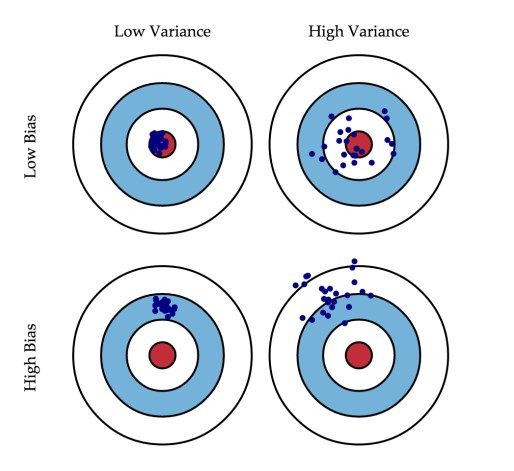
\includegraphics[width=1\textwidth]{img/bias_var.jpg}
	\caption{Сдвиг и разброс разных моделей}
	\label{fig:bias_var}
\end{figure}


На рис. \ref{fig:bias_var} изображены модели с различными сдвигом и разбросом. Модели изображены синими точками, одна точка соответствует модели, обученной по одной из возможных обучающих выборок. Каждый круг характеризует качество модели --- чем ближе точка к центру, тем меньше ошибок на контрольной выборке достигает данный алгоритм. Видно, что большой сдвиг соответствует тому, что в среднем точки не попадают в центр, то есть в среднем они не соответствуют лучшей модели.

Большой разброс означает, что модель может попасть по качеству куда угодно --- как в центр, так и в область с большой ошибкой.

\section{Bagging}

Деревья решений, страдают от высокой дисперсии. Это означает, что если разделить обучающие данные на две части случайным образом и применить дерево решений к обеим половинам, результаты, которые мы получим, могут быть совершенно разными. Напротив, процедура с низкой дисперсией даст схожие результаты при многократном применении к разным наборам данных; линейная регрессия имеет тенденцию к низкой дисперсии, если отношение $n$ к $p$ умеренно велико. Бэггинг, --- это процедура для уменьшения дисперсии статистического метода обучения; она особенно полезна и часто используется в контексте деревьев решений.

Пусть у нас имеется набор из $n$ независивых наблюдений $X_1,\ldots X_n$, каждый из которых имеет дисперсию $\sigma^2$, дисперсия $\bar{X}$ будет равна $\sigma^2/n$. Другими словами, усреднение набора наблюдений снижает дисперсию.

Следовательно, естественный способ уменьшить дисперсию и, следовательно, увеличить точность предсказания статистического метода обучения заключается в том, чтобы взять множество обучающих наборов из выборки, построить отдельную модель предсказания, используя каждый набор обучения и усреднить полученные прогнозы. 

\begin{equation}
	{a}_{N}(x) = \dfrac{1}{N}\sum_{n=1}^{N}\hat{\mu}(x)
\end{equation}

Однако на практике это не реализовать, потому что у нас нет нескольких сетов обучающих данных. Вместо этого, мы можем примеить бутстрап беря несколько сэмплов из обучающего набора данных. При таком подходе, мы генерируем $B$ разных подвыборок с помощью бутсрапа. Затем мы обучаем модель на $b$-ом сете обучающих данных и усредняем прогнозы.

Это называется бэггингом.

Заметим, что в методе обучения для бэггинга появляется ещё один источник случайности — взятие подвыборки. Чтобы функционал качества $L(\mu)$ был детерминированным, мы будем далее считать, что матожидание$ \mathbb{E}_X [\cdot]$ берётся не только по всем обучающим выборкам $ X$, но ещё и по всем возможным подвыборкам $\hat{X}$, получаемым с помощью бутстрапа. Это вполне логичное обобщение, поскольку данное матожидание вводится в функционал именно для учёта случайностей, связанных с процедурой обучения модели.

Найдём смещение из разложения (\ref{2.4}) для бэггинга:

\begin{multline}
	\mathbb{E}_{x,y}\left[\left(\mathbb{E}_X\left[\frac{1}{N}\sum_{b=1}^{N}\hat{\mu}(X)(x)\right]-\mathbb{E}[y|x]\right)^2\right] = \mathbb{E}_{x,y}\left[\left(\frac{1}{N}\sum_{b=1}^{N}\mathbb{E}_X[\hat{\mu}(X)(x)] - \mathbb{E}[y|x]\right)^2\right] = \\ =\mathbb{E}_{x,y}\left[(\mathbb{E}_X\left[\hat{\mu}(X)(x)\right]-\mathbb{E}[y|x])^2\right]
\end{multline}


Мы получили, что смещение композиции, полученной с помощью бэггинга, совпадает со смещением одного базового алгоритма. Таким образом, бэггинг не ухудшает смещенность модели.

Теперь рассмотрим разброс. Из (\ref{2.4}) он равен:

\begin{multline}
	\frac{1}{N}\mathbb{E}_{x,y}\left[\mathbb{E}_X\left[\left(\hat{\mu}(X)(x)-\mathbb{E}_X[\hat{\mu}(X)(x)]\right)^2\right]\right] + \\ + 
	\frac{N(N-1)}{N^2}\mathbb{E}_{x,y}\left[\mathbb{E}_X\left[\left(\hat{\mu}(X)(x)-\mathbb{E}_X[\hat{\mu}(X)(x)]\right)\times \left(\hat{\mu}(X)(x)-\mathbb{E}_X[\hat{\mu}(X)(x)]\right)\right]\right]
\end{multline}

Первое слагаемое — это дисперсия одного базового алгоритма, деленная на длину композиции $N.$ Второе --- ковариация между двумя базовыми алгоритмами. Мы видим, что если базовые алгоритмы некоррелированы, то дисперсия композиции в $N$ раз меньше дисперсии отдельных алгоритмов. Если же корреляция имеет место, то уменьшение дисперсии может быть гораздо менее существенным.

До сих пор мы описывали бэггинг в контексте регрессии, для предсказания количественного результата $y$. Как можно распространить бэггинг на задачу классификации, где $Y$ является качественным? В этой ситуации существует существует несколько возможных подходов, но самый простой заключается в следующем. Для тестового сета, мы можем записать класс, предсказанный каждым из $N$ деревьев, и сделать "\textit{majority vote}" --- это наиболее часто встречающийся класс среди $N$ предсказаний.

\subsection{Out-of-Bag Error Estimation}

Ключевой момент bagging модели заключается в том, что деревья многократно подгоняются к бутстреп-подмножествам наблюдений. В среднем каждое дерево сетки использует около двух третей наблюдений. Оставшаяся треть наблюдений, не использованная для подгонки данного дерева сетки, называется \textit{out-of-bag} наблюдениями (OOB).

Мы можем предсказать ответ для i-го наблюдения, используя каждое из деревьев, в которых это наблюдение было OOB. Это даст около N/3 предсказаний для i-го наблюдения. Для того чтобы получить единое предсказание для i-го  наблюдения, мы можем усреднить эти предсказанные ответы (при регрессионной модели) или взять majority vote (при классификации). Это приводит к единственному OOB-предсказанию для каждого наблюдения. Предсказание OOB может быть получено таким образом для каждого из $n$ наблюдений, из чего следует, что общий MSE OOB (для задачи регрессии) или ошибка классификации (для задачи классификации) может быть вычислена. Полученная ошибка OOB является достоверной оценкой тестовой ошибки для bagging модели, поскольку прогноз для каждого наблюдения предсказывается с использованием только тех деревьев, которые не подошли для данного наблюдения. 

$OOB = \sum_{i=1}^{l}L\left(y_i,\frac{1}{\sum_{n=1}^{N}\left[x_i \notin X_n\right]}\sum_{n=1}^{N}[x_i\notin X_n]b_n(x_i)\right)$

\subsection{Значимость переменных}

Как говорилось ранее, бэггинг обычно приводит к повышению точности по сравнению с предсказанием с помощью одного дерева. Однако, к сожалению, интерпретировать полученную модель может быть сложно. Напомним, что одним из преимуществ деревьев решений является привлекательная и легко интерпретируемая диаграмма, которая получается в результате. Однако, когда мы объединяем большое количество деревьев, уже невозможно представить результирующую процедуру статистического обучения с помощью одного дерева, и уже не ясно, какие переменные являются наиболее важными для процедуры. Таким образом, группировка деревьев повышает точность прогнозирования точность прогноза за счет интерпретируемости. 

Хотя набор деревьев построенных с помощью бэггинга гораздо сложнее интерпретировать чем отдельное дерево, можно получить общую сводку важности каждого предиктора, используя RSS (для деревьев регрессии) или индекс Джини (для деревьев классификации). В случае  деревьев регрессии, мы можем записать общую сумму, на которую RSS уменьшается из-за разделяется для данного предиктора, усредненное по всем $B$ деревьям. Большое значение указывает на важный предиктор. Аналогично, в контексте  классификации деревьев, мы можем сложить общую сумму, на которую индекс Джини  уменьшается в результате разделения по заданному предиктору, в среднем по всем B-деревьям.


\section{Random Forest}

Бэггинг позволяет объединить несмещенные, но чувствительные к обучающей выборке алгоритмы в несмещенную композицию с низкой дисперсией. Хорошим семейством базовых алгоритмов здесь являются решающие деревья --- они достаточно сложны и могут достигать нулевой ошибки на любой выборке (следовательно, имеют низкое смещение), но в то же время легко переобучаются.

Метод случайных лесов основан на бэггинге над решающими деревьями.

\textbf{Алгоритм:}
Ддля $n=1,\ldots,N$
\begin{enumerate}
	\item Сгенерировать выборку $\hat{X}_n$ с помощью бутстрапа.
	\item Построить решающее дерево $b_n(x)$ по выборке $\hat{X}_n$.
	\begin{itemize}
		\item дерево строится, пока в каждом листе не окажется не более $n_{min}$ объектов
		\item при каждом разбиении сначала выбирается $m$ случайных признаков из $p$ и оптимальное разделение ищется только среди них
	\end{itemize}
	\item Вернуть композицию $a_N(x) = \dfrac{1}{N}\sum_{n=1}^{N}b_n(x)$
\end{enumerate}

В случайных лесах корреляция между деревьями понижается путем рандомизации по двум направлениям: по объектам и по признакам. Во-первых, каждое дерево обучается по бутстрапированной подвыборке. Во-вторых, в каждой вершине разбиение ищется по подмножеству признаков. Вспомним, что при построении дерева последовательно происходит разделение вершин до тех пор, пока не будет достигнуто идеальное качество на обучении. Каждая вершина разбивает выборку по одному из признаков относительно некоторого порога. В случайных лесах признак, по которому производится разбиение, выбирается не из всех возможных признаков, а лишь из их случайного подмножества размера $m$.

Рекомендуется в задачах классификации брать $m=\sqrt{p}$, а в задачах регрессии --- $m=p/3$. Также рекомендуется в задачах классификации строить каждое дерево до тех пор, пока в каждом листе не окажется по одному объекту, а в задачах регрессии — пока в каждом листе не окажется по пять объектов. 

Случайные леса --- один из самых сильных методов построения композиций. На практике он может работать немного хуже градиентного бустинга, но при этом он гораздо более прост в реализации.

\section{Boosting}

Ранее мы изучили бэггинг и случайные леса — подходы к построению композиций, которые независимо обучают каждый базовый алгоритм по некоторому подмножеству обучающих данных. При этом возникает ощущение, что мы используем
возможности объединения алгоритмов не в полную силу, и можно было бы строить их так, чтобы каждая следующая модель исправляла ошибки предыдущих. Ниже мы рассмотрим метод, который реализует эту идею — градиентный бустинг. Он работает для любых дифференцируемых функций потерь и является одним из наиболее мощных и универсальных на сегодняшний день.

\subsection{Бустинг в задаче регрессии}

Рассмотрим задачу минимизации квадратичного функционала:

$\dfrac{1}{2}\sum_{i=1}^{l}(a(x_i)-y_i)^2 \rightarrow \underset{a}{min}$

Будем искать итоговый алгоритм в виде суммы базовых моделей $b_n(x)$:

$a_N(x) = \sum_{n=1}^{N}b_n(x)$, где базовые алгоритмы $b_n$ принадлежат некоторому семейству $\mathbf{A}$.

Первый базовый алгоритм: $b_1(x):= \underset{b\in\mathbf{A}}{argmin} \dfrac{1}{2}\sum_{i=1}^{l}(b(x_i)-y_i)^2$.

Решение такой задачи не представляет трудностей для многих семейств алгоритмов. Теперь мы можем посчитать остатки на каждом обхекте --- растояния от ответа нашего алгоритма до истинного ответа: $s^{(1)}_i = y_i - b_i(x)$

Если прибавить эти остатки к ответам построенного алгоритма, то он не будет допускать ошибок на обучающей выборке. Значит, будет разумно построить второй алгоритм так, чтобы его ответы были как можно ближе к остаткам:

$b_2(x) := \underset{b\in\mathbf{A}}{argmin} \dfrac{1}{2}\sum_{i=1}^{l}(b(x_i)-s^{(1)})^2$

Таким образом, каждый следующий алгоритм тоже будем настраивать на остатки предыдущих:

$s^{(N)}_i = y_i - \sum_{n=1}{N-1}b_n(x_i) = y_i - a_{N-1}(x_i),\qquad i=1,\ldots,l$

$b_N(x):= \underset{b\in\mathbf{A}}{argmin} \dfrac{1}{2}\sum_{i=1}^{l}(b(x_i)-s_i^{(N)})^2$

Также, остатки могут быть найдены как антиградиент функции потерь по ответу модели, посчитанный в точке ответа уже построенной композиции:

$s_i^{(N)} = y_i - a_{N-1}(x_i)= \left.- \diffp{}{z}\dfrac{1}{2}(z-y_i)^2\right|_{z=a_{N-1}(x_i)}$

Получается, что выбирается такой базовый алгоритм, который как можно сильнее уменьшит ошибку композиции — это свойство вытекает из его близости к антиградиенту функционала на обучающей выборке.

\subsection{Градиентный бустинг}

Пусть дана некоторая дифференцируемая функция потерь $L(y, z)$. Будем строить взвешенную сумму базовых алгоритмов:

$a_N(x) = \sum_{n=0}^{N}\gamma_n b_n(x)$

Заметим, что в композиции имеется начальный алгоритм $b_0(x)$. Как правило, коэффициент $\gamma_0$ при нем берут равным единице, а сам алгоритм выбирают очень простым.

\textbf{Примеры выбора алгоритма $b_0(x)$:}

\begin{enumerate}
	\item Нулевой: $b_0(x) = 0$.
	\item Возвращающий самый популярный класс (в задачах классификации):
	
	$b_0(x) = \underset{y\in\mathbf{\mathbb{Y}}}{argmax}\sum_{i=1}^{l}[y_i=y]$
	\item Возвращающий средний ответ (в задачах регрессии):	
	$b_0(x) = \frac{1}{l}\sum_{i=1}{l}y_i$
\end{enumerate}

Допустим, мы построили композицию $a_{N-1}(x)$ из $N-1$ алгоритма, и хотим выбрать следующий абзовый алгоритм $b_N(x)$ так, чтобы как можно сильнее уменьшить ошибку:

$\sum_{i=1}^{l} L\left(y_i,a_{N-1}(x_i) + \gamma_N b_N(x_i)\right)\rightarrow \underset{b_N,\gamma_N}{min}$

Ответим в первую очередь на следующий вопрос: если бы в качестве алгоритма $b_N (x)$ мы могли выбрать совершенно любую функцию, то какие значения ей следовало бы принимать на объектах обучающей выборки? Иными словами, нам нужно понять, какие числа $s_1,\ldots, s_l$ надо выбрать для решения следующей задачи:

$\sum_{i=1}^{l} L\left(y_i, a_{N-1}(x_i) +s_i\right)\rightarrow \underset{s_1,\ldots, s_l}{min}$

Можно, например, выбрать $s_i = y_i - a_{N-1}(x_i)$, но данный подход не учитывает особенностей функции потерть $L(y,z)$.

Другой вариант --- потребовать чтобы сдвиг $s_i$ был противоположен производной функции потерь в точке $z=a_{N-1}(x_i)$:

$s_i = -\left. \diffp{L}{z} \right|_{z=a_{N-1}(x_i)}$

В таком случае мы сдвинемся в сторону скорейшего убывания функции потерь. Заметим, что вектор сдвигов $s = s_1,\ldots, s_l$ совпадает с антиградиентом:

$\left(\left. -\diffp{L}{z}\right|_{z=a_{N-1}(x_i)}\right)^l_{i=1} = -\bigtriangledown_z \sum_{i=1}^{l}\left. L(y_i,z_i) \right|_{z=a_{N-1}(x_i)}$

При таком выборе сдвигов $s_i$ мы, по сути, сделаем один шаг градиентного спуска, двигаясь в сторону наискорейшего убывания ошибки на обучающей выборке. Отметим, что речь идет о градиентном спуске в $l$-мерном пространстве предсказаний алгоритма на объектах обучающей выборки. Поскольку вектор сдвига будет свой на
каждой итерации, правильнее обозначать его как $s_i^{(N)}$, но для простоты будем иногда
опускать верхний индекс.

Итак, мы поняли, какие значения новый алгоритм должен принимать на объектах обучающей выборки. По данным значениям в конечном числе точек необходимо построить функцию, заданную на всем пространстве объектов. Это классическая задача обучения с учителем, которую мы уже хорошо умеем решать. Один из самых простых функционалов --- среднеквадратичная ошибка. Воспользуемся им для поиска базового алгоритма, приближающего градиент функции потерь на обучающей выборке:


$b_N(x) = \underset{b\in\mathbf{A}}{argmin}\sum_{i=1}^{l} (b(x_i) - s_i)^2$

После того, как новый базовый алгоритм найден, можно подобрать коэффициент при нем по аналогии с наискорейшим градиентным спуском:

$\gamma_N = \underset{\gamma\in\mathbf{\mathbb{R}}}{argmin}\sum_{i=1}^{l} L(y_i,a_{N-1}(x_i) + \gamma b_N(x_i))$

Описанный подход с аппроксимацией антиградиента базовыми алгоритмами и называется градиентным бустингом. Данный метод представляет собой поиск лучшей функции, восстанавливающей истинную зависимость ответов от объектов, в пространстве всех возможных функций. Ищем мы данную функцию с помощью «псевдоградиентного» спуска --- каждый шаг делается вдоль направления, задаваемого некоторым базовым алгоритмом. При этом сам базовый алгоритм выбирается так, чтобы как можно лучше приближать антиградиент ошибки на обучающей выборке.

\subsection{Регуляризация}

\subsubsection{Сокращение шага}

На практике оказывается, что градиентный бустинг очень быстро строит композицию, ошибка которой на обучении выходит на асимптоту, после чего начинает настраиваться на шум и переобучаться. Это явление можно объяснить одной из двух причин:

\begin{itemize}
	\item Если базовые алгоритмы очень простые (например, решающие деревья небольшой глубины), то они плохо приближают вектор антиградиента. По сути, добавление такого базового алгоритма будет соответствовать шагу вдоль направления, сильно отличающегося от направления наискорейшего убывания. Соответственно, градиентный бустинг может свестись к случайному блужданию в
	пространстве
	\item Если базовые алгоритмы сложные (например, глубокие решающие деревья), то они способны за несколько шагов бустинга идеально подогнаться под обучающую выборку — что, очевидно, будет являться переобучением, связанным с излишней сложностью семейства алгоритмов.
\end{itemize}

Сокращение шага представляет собой следующее: вместо перехода в оптимальную точку в направлении антиградиента
делается укороченный шаг

$a_N(x) = a_{N-1}(x) + \eta\gamma_Nb_N(x)$,

где $\eta \in (0,1]$ --- темп обучения. Как правило, чем меньше темп обучения, тем лучше качество итоговой композиции. Сокращение шага, по сути, позволяет понизить доверие к направлению, восстановленному базовым алгоритмом.

Также следует обратить внимание на число итераций градиентного бустинга. Хотя ошибка на обучении монотонно стремится к нулю, ошибка на контроле, как правило, начинает увеличиваться после определенной итерации. Оптимальное число итераций можно выбирать, например, по отложенной выборке или с помощью кроссвалидации.


\subsubsection{Стохастический градиентный бустинг}

Еще одним способом улучшения качества градиентного бустинга является внесение рандомизации в процесс обучения базовых алгоритмов. А именно, алгоритм $b_N$ обучается не по всей выборке $X$, а лишь по ее случайному подмножеству $X^k \subset X$. В этом случае понижается уровень шума в обучении, а также повышается эффективность вычислений. Существует рекомендация брать подвыборки, размер которых вдвое меньше исходной выборки.

\subsection{Функции потерь}

\subsubsection{Регрессия}

Одна ищ функций потерь --- квадратичная, была рассмотрена в разделе 6.1. Другой вариант --- модуль отклонения $L(y,z) = |y-z|$, для которого антиградиент вычисляется по формуле 

$s_i^{(N)} = -sign(a_{N-1}(x_i)-y_i)$

\subsubsection{Классификация}

В задаче классификации с двумя классами разумным выбором является логистическая функция потерь:

$L(y,z) = log(1+exp(-yz))$

Задача поиска базового алгоритма с ней принимает вид

$b_N = \underset{b\in\mathbf{A}}{argmin}\sum_{i=1}^{l} (b(x_i) - \frac{y_i}{1+exp(y_ia_{N-1}(x_i))})^2$

Логистическая функция потерь имеет интересную особенность, связанную со взвешиванием объектов. Заметим, что ошибка на $N$-й итерации может быть записана как

$Q(a_N) = \sum_{i=1}^{l}log(1+exp(-y_ia_N(x_i))) = \sum_{i=1}^{l}log(1+exp(-y_ia_{N-1}(x_i))exp(-y_i \gamma_n b_N(x_i)))$

Если отступ $y_ia_{N-1}(x_i)$ на $i$-м объекте большой положительный, то данный объект не будет вносить практически никакого вклада в ошибку, и может быть исключен из всех вычислений на текущей итерации без потерь.

Таким образом, величина $w_i^{(N)} = exp(-y_ia_{N-1}x(i))$ можем случить мерой важности объекта $x_i$ на $N$-й итерации градиентного бустинга.


\subsection{Градиентный бустинг над деревьями}

Считается, что градиентный бустинг над решающими деревьями --- один из самых универсальных и сильных методов машинного обучения, известных на сегодняшний день.

Как известно, решающее дерево разбивает все пространство на непересекающиеся области, в каждой из которых его ответ равен константе $b_n(x) = \sum_{j=1}^{J_n} b_{nj}[x\in R_j]$, где $j=1,\ldots,J_n$ --- индексы листьев, $R_{j}$ --- соответствующие области разбиения, $b_{nj}$ --- значения в листьях. Значит в $N$-й итерации бустинга композиция обновляется как

$a_N(x) = a_{N-1}(x) + \gamma_N \sum_{j=1}^{J_N}b_{Nj}[x\in R_j]$.

Видно, что добавление в композицию одного дерева с $J_N$ листьями равносильно добавлению $J_N$ базовых алгоритмов, представляющих собой предикаты. Мы можем улучшить качество композиции, подобрав свой коэффициент при каждом из предикатов: 

$\sum_{i=1}^{l} L\left(y_i,a_{N-1}(x_i) + \sum_{j=1}^{J_N} \gamma_{Nj}[x\in R_j]\right) \rightarrow \underset{\left\{\gamma_{Nj}\right\}^{J_N}_{j=1}}{min}$

Так как области разбиения $R_j$ не пересекаются, данная задача распадается на $J_N$ независимых подзадач:

$\gamma_{Nj} = \underset{\gamma}{argmin} \sum_{x_i \in R_j} L(y_i, a_{N-1}(x_i) + \gamma), \qquad j=1,\ldots J_N$

В некоторых случаях оптимальные коэффициенты могут быть найдены аналитически --- например, для квадратичной и абсолютной ошибки.

Рассмотрим теперь логистическую функцию потерь. В этом случае нужно решить задачу
$F_j^{(N)}(\gamma) = \sum_{x_i \in R_j} log(1 + exp(-y_i(a_{N-1}(x_i) + \gamma))) \rightarrow \underset{\gamma}{min}$.

Данная задача может быть решена лишь с помощью итерационных методов, аналитической записи для оптимального $\gamma$ не существует. Однако на практике обычно нет необходимости искать точное решение — оказывается достаточным сделать лишь один шаг метода Ньютона-Рафсона из начального приближения $\gamma_{Nj} = 0$. 

\subsubsection{Смещение и разброс}

В случайных лесах используются глубокие деревья, поскольку от базовых алгоритмов требуется низкое смещение; разброс же устраняется за счёт усреднения ответов различных деревьев. Бустинг работает несколько иначе — в
нём каждый следующий алгоритм целенаправленно понижает ошибку композиции, и даже при использовании простейших базовых моделей композиция может оказаться достаточно сложной. Более того, итоговая композиция вполне может оказаться переобученной при большом количестве базовых моделей. Это означает, что благодаря бустингу можно понизить смещение моделей, а разброс либо останется таким же, либо увеличится. Из-за этого, как правило, в бустинге используются неглубокие решающие деревья (3-6 уровней), которые обладают большим смещением, но не
склонны к переобучению.

\subsection{Взвешивание объектов}

Одним из первых широко распространённых методов построения композиций является AdaBoost, в котором оптимизируется экспоненциальная функция потерь $L(y,z)= exp(-yz)$. Благодаря её свойствам удаётся свести задачу поиска базового алгоритма к минимизации доли неверных ответов с весами при объектах. Эти веса возникают и в градиентном бустинге при использовании экспоненциальной функции потерь:

$L(a,X) = \sum_{i=1}^{l} exp\left(-y_i\sum_{n=1}^{N}\gamma_nb_n(x_i)\right)$

Компоненты ее антиградиента после $N-1$ итерации:

$s_i=\left. -\diffp{L(y_i,z)}{z}\right|_z=a_{N-1}(x_i)$ $=y_i\underbrace{exp\left(-y_i\sum_{n=1}^{N-1}\gamma_nb_n(x_i)\right)}_{w_i}$

Заметим, что антиградиент представляет собой ответ на объекте, умноженный на его вес. Если все веса будут равны единице, то следующий базовый классификатор будет просто настраиваться на исходный целевой вектор $(y_i)^l_{i=1}$;штраф за выдачу ответа, противоположного правильному, будет равен 4 (поскольку при настройке базового алгоритма используется квадратичная функция потерь). Если же какой-либо объект будет иметь большой отступ, то его вес окажется близким к нулю, и штраф за выдачу любого ответа будет равен 1.

\subsection{Влияние шума на обучение}

Выше мы находили формулу для антиградиента при использовании экспоненциальной функции потерь:

$s_i=y_i\underbrace{exp\left(-y_i\sum_{n=1}^{N-1}\gamma_nb_n(x_i)\right)}_{w_i}$.

Заметим, что если отступ на объекте большой и отрицательный (что обычно наблюдается на шумовых объектах), то вес становится очень большим, причем он никак не ограничен сверху. В результате базовый классификатор будет настраиваться исключительно на шумовые объекты, что может привести к неустойчивости его ответов и переобучению.
Рассмотрим теперь логистическую функцию потерь, которая также может использоваться в задачах классификации:

$L(a,X^l) = \sum_{i=1}^{l}log(1+exp(-y_ia(x_i)))$

Ее антиградиент после $N-1$ шага:

$s_i = y_i \underbrace{\frac{1}{1+exp(y_ia_{N-1}(x_i))}}_{w_i^{(N)}}$

Теперь веса ограничены сверху единицей. Если отступ на объекте большой отрицательный (то есть это выброс), то вес при нем будет близок к единице; если же отступ на объекте близок к нулю (то есть это объект, на котором классификация неуверенная, и нужно ее усиливать), то вес при нем будет примерно равен 1/2. Таким образом,
вес при шумовом объекте будет всего в два раза больше, чем вес при нормальных объектах, что не должно сильно повлиять на процесс обучения.


\end{document}